\documentclass[12pt,a4paper]{article}

\def\version{6.4}

\def\qe{{\sc Quantum ESPRESSO}}
\sloppy
\usepackage{html}

% BEWARE: don't revert from graphicx for epsfig, because latex2html
% doesn't handle epsfig commands !!!
\usepackage{graphicx}
\usepackage{upquote}
\usepackage{color}
\usepackage[usenames,dvipsnames,svgnames,table]{xcolor}

\textwidth = 17cm
\textheight = 24cm
\topmargin =-1 cm
\oddsidemargin = 0 cm

\def\pwx{\texttt{pw.x}}
\def\cpx{\texttt{cp.x}}
\def\phx{\texttt{ph.x}}
\def\ppx{\texttt{pp.x}}
\def\nebx{\texttt{neb.x}}
\def\configure{\texttt{configure}}
\def\PWscf{\texttt{PWscf}}
\def\PHonon{\texttt{PHonon}}
\def\CP{\texttt{CP}}
\def\PostProc{\texttt{PostProc}}
\def\NEB{\texttt{PWneb}}
\def\make{\texttt{make}}
%\def\QEmodes{\texttt{QE-emacs-modes}}
\def\QEmodes{\texttt{QE-modes}}
\def\QEemodes{\texttt{QE-emacs-modes}}
\def\qemodes{\texttt{qe-modes}}

\def\efn#1{\textcolor{BlueViolet}{\texttt{#1}}}
\def\var#1{\textcolor{Blue}{\texttt{\textit{#1}}}}
\def\bvar#1{\texttt{\textit{#1}}}

\def\qemode{\efn{qe-mode}}
\def\nebmode{\efn{neb-mode}}
\def\pwmode{\efn{pw-mode}}
\def\cpmode{\efn{cp-mode}}
\def\phmode{\efn{ph-mode}}
\def\ldmode{\efn{ld1-mode}}
\def\ppmode{\efn{pp-mode}}
%\def\prmode{\efn{projwfc-mode}}

\begin{document} 
\author{}
\date{}

\def\qeImage{../../../Doc/quantum_espresso.pdf}

\title{
  \includegraphics[width=5cm]{\qeImage} \\
  % title
  \Huge \QEemodes\ User's Guide (v.\version) 
}

\maketitle

\tableofcontents

\section{Introduction}

This guide covers the usage of \QEemodes\ package (aka \QEmodes): an
open-source collection of Emacs major-modes for making the editing of
\qe\ (QE) input files somewhat easier and more comfortable with Emacs
editor. The package provides syntax highlighting (see
Figure~\ref{fig:example}), basic auto-indentation, and several utility
commands.

\section{Terms of use}

\QEmodes\ is free software, released under the
GNU General Public License. See:
\texttt{http://www.gnu.org/licenses/old-licenses/gpl-2.0.txt}, or the
file \texttt{License} in the \qe\ distribution.

The \QEmodes\ package was written by Anton Kokalj. The implementation
of \QEmodes\ was made possible by several useful and helpful resources
that are gratefully acknowledged, in particular: {\it Mode Tutorial}
of Scott Andrew Borton
(\texttt{https://www.emacswiki.org/emacs/ModeTutorial} for
indentation code), {\it Derived Mode} and {\it Sample Mode} pages
(\texttt{https://www.emacswiki.org/emacs/DerivedMode},
\texttt{https://www.emacswiki.org/emacs/SampleMode}) as well as the
very useful resources of Xah Lee
(\texttt{http://ergoemacs.org/emacs/elisp\_syntax\_coloring.html}). Last
but not the least Sebastijan Peljhan is acknowledged for his work on
\texttt{xsf-mode} that inspired the idea of writing the \QEmodes.

% TODO: add infro from the net.

\begin{figure}[htb]
  \centering
  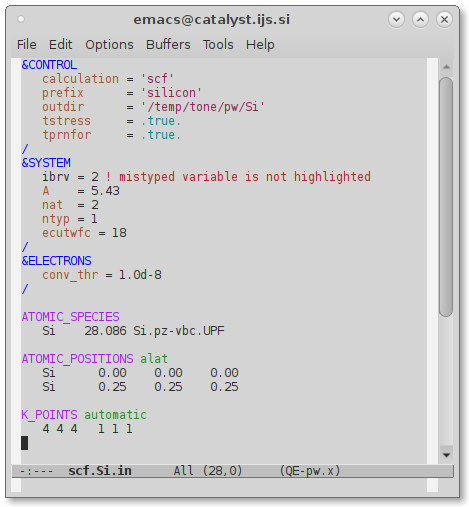
\includegraphics[width=0.8\textwidth]{highlight.png}
  \caption{A \pwx\ input file opened with \pwmode\ in Emacs. Note the
    highlighted elements: namelists and their variables (blue and
    brown), cards and their flags (purple and green), comments (red),
    string and logical variable values (burgundy and cyan,
    respectively). Note that mistyped variable (i.e.\ \texttt{ibrv}
    instead of \texttt{ibrav}) is not highlighted.}
  \label{fig:example}
\end{figure}
    
\section{Installation}

The installation of \QEmodes\ package consists of two parts: (i)
installing the package itself and (ii) informing Emacs about it by
editing the \verb+user-init-file+ (typically \verb+$HOME/.emacs+).

\subsection{Installing the \QEmodes\ package}
Once the \texttt{QE-modes-\version.tar.gz} archive is unpacked and you
are located in its root directory, the installation is trivial. Simply
copy the whole \qemodes\ subdirectory to appropriate place. To
facilitate this copying on Unix-like operating systems, one can use:
\begin{verbatim}
   ./install.sh
\end{verbatim}
which will install the package in the \qemodes\ subdirectory of the
\texttt{\$HOME/.emacs.d/} directory. If you prefer to install it into
other directory, then use:
\begin{flushleft}
\verb+   prefix=+\var{where-to-install}\verb+ ./install.sh+
\end{flushleft}
which will install the package in the \qemodes\ subdirectory of
\var{where-to-install} directory.

% \paragraph{Note for non-Unix operating systems:} Given that
% \texttt{install.sh} is a shell script its execution may fail on
% non-Unix operating systems. In this case manually copy the \qemodes/
% subdirectory to appropriate place.

\subsection{Editing the \texttt{user-init-file} file}

An example snippet of \texttt{user-init-file} for \QEmodes\ is
provided by the \texttt{qe-modes.emacs} file in the package root
directory and the text below explains it. In particular, to use the
installed \QEmodes\ in Emacs, add the following to your
\verb+user-init-file+ (e.g.\ \verb+$HOME/.emacs+):
\begin{flushleft}
{\color{red}
\verb+   ;; make sure package is visible to emacs (if needed)+}\\
\verb+   (add-to-list 'load-path "+\var{/full/path/name/of}\verb+/qe-modes")+\\[1em]
{\color{red}
\verb+   ;; load the package+}\\
\verb+   (require 'qe-modes)+
\end{flushleft}
where \var{/full/path/name/of} is the directory where the \qemodes\
are installed (either the \texttt{\$HOME/.emacs.d/} or the above
\var{where-to-install}).


Furthermore, we can specify some filename patterns so that Emacs will
automatically recognize from the filename if it is some variant of the
\qe\ input file.
%
Say that we use the \verb+.in+ extension for the \qe\ input files in
general and more specifically, the \texttt{pw.}, \texttt{scf.},
\texttt{relax.}, and \texttt{vc-relax.} prefixes for the \pwx\ input files
and \texttt{neb.}, \texttt{ph.},  and \texttt{pp.} prefixes for the
\nebx, \phx, and \ppx\ input files. These filename recognitions can be
achieved by:
\begin{flushleft}
{\color{red}
\verb+   ;; automatically open the *.in files with generic QE mode+}\\
\verb+   (add-to-list 'auto-mode-alist  '("\\.in\\'" . qe-mode))+\\[1em]
{\color{red}
\verb+   ;; automatically open the pw*.in, scf*.in, relax*in, vc-relax*.in files+\\
\verb+   ;; with pw.x mode+}\\
\verb+   (add-to-list 'auto-mode-alist  '("pw.*\\.in\\'" . pw-mode))+\\
\verb+   (add-to-list 'auto-mode-alist  '("scf.*\\.in\\'" . pw-mode))+\\
\verb+   (add-to-list 'auto-mode-alist  '("relax.*\\.in\\'" . pw-mode))+\\
\verb+   (add-to-list 'auto-mode-alist  '("vc-relax.*\\.in\\'" . pw-mode))+\\[1em]
{\color{red}
\verb+   ;; automatically open the neb*.in files with neb.x mode+}\\
\verb+   (add-to-list 'auto-mode-alist  '("neb.*\\.in\\'" . neb-mode))+\\[1em]
{\color{red}
\verb+   ;; automatically open the ph*.in files with ph.x mode+}\\
\verb+   (add-to-list 'auto-mode-alist  '("ph.*\\.in\\'" . ph-mode))+\\[1em]
{\color{red}
\verb+   ;; automatically open the pp*.in files with pp.x mode+}\\
\verb+   (add-to-list 'auto-mode-alist  '("pp.*\\.in\\'" . pp-mode))+\\[1em]
\end{flushleft}
Beware that the more general \texttt{*.in} pattern for the generic
\qemode\footnote{Please note the difference between \qemodes\ and
  \qemode: the first implies the whole package, whereas the second
  means the generic QE mode, which is only one among the available
  modes in the \qemodes\ package.} should be specified first
or else any \texttt{*.in} file will be recognized as generic QE input
file.

For those who are fans of regular-expressions, the above four lines
for \pwmode\ can be expressed by the following one-liner:

{\footnotesize
  \begin{verbatim}
   (add-to-list 'auto-mode-alist '("\\(pw\\|scf\\|\\(?:vc-\\)?relax\\).*\\.in\\'" . pw-mode))
\end{verbatim}
}

Once the package is installed according to the above instructions, we
are ready to use it. Let us, for the sake of example, open an existing
\texttt{pw.x} input file whose name does not match the above specified
filename pattern for the \pwmode. In such cases we can load the mode
with \efn{M-x pw-mode} command and we will get the content of the file
highlighted as in Figure~\ref{fig:example}.

\section{Usage}

\subsection{Available modes defined by \qemodes}

The \QEmodes\ package contains a generic \qemode\ and the following
specific modes: \pwmode, \nebmode, \cpmode, \phmode, \ldmode, and \ppmode.
%\subsubsection{Difference between generic \qemode\ and specific modes}
The difference between them is only in the extent of the syntax
highlighting and auto-indentation. Namely, these modes recognize and
highlight namelists (and their variables) and cards (and their
options/flags) that they know about.
%
The generic \qemode\ is aware of all of them for all those \qe\
programs that have explicit documentation in the form of
\verb+INPUT_+\var{PROG}\verb+.html+ files (where \var{PROG}
typically stands for the uppercase name of the program). In contrast,
a given specific mode is aware only of namelists, variables, cards, and
options of the corresponding program.

\begin{figure}[htb]
  \centering
  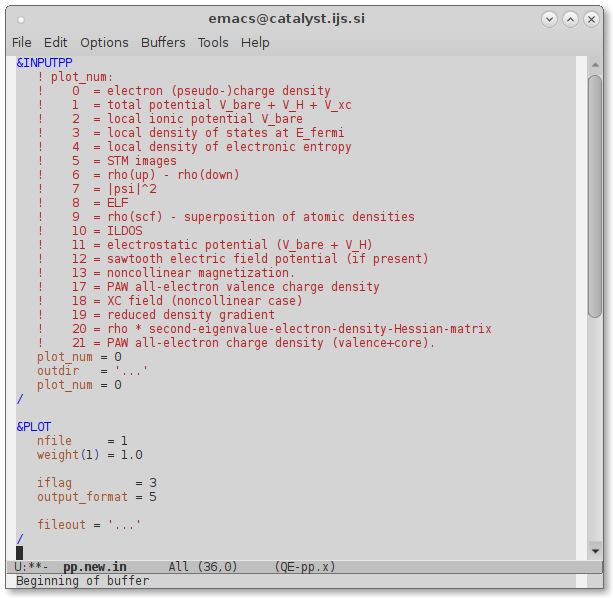
\includegraphics[width=0.8\textwidth]{insert-template.png}
  \caption{The result of executing the \efn{M-x pp-insert-template}
    command, which insert a template for the \ppx\ input file into the
    current buffer.}
  \label{fig:insert-template}
\end{figure}
\subsection{Commands}

The \QEmodes\ package provides the following commands:
\begin{description}
\item[$\bullet$ \efn{M-X \var{mode}-mode}]\hfill\\ toggles
  the respective mode, where \var{mode} is one of \texttt{qe},
  \texttt{pw}, \texttt{neb}, \texttt{cp}, \texttt{ph}, \texttt{ld1}, or \texttt{pp}

\item[$\bullet$ \efn{M-x indent-region}] ~~{\rm or}~~ \efn{C-M-\textbackslash}\hfill\\
  indents region according to \qemodes\ rules, i.e., namelist and card
  names are left aligned to the first column, while their content is
  indented by \texttt{qe-indent} spaces to the right (see
  Figure~\ref{fig:example}; default value of \texttt{qe-indent} is 3)

\item[$\bullet$ \efn{M-x \var{prog}-insert-template}]\hfill\\
  inserts a respective input file template (see Figure 2); this
  command may not be defined for all the \var{prog}s; currently
  supported \var{prog}s are: \texttt{pw}, \texttt{pp}, \texttt{neb},
  \texttt{ph}, \texttt{dynmat}, \texttt{ld1}, \texttt{projwfc},
  \texttt{dos}, and \texttt{bands}.

\item[$\bullet$ \efn{M-x \var{prog-NAMELIST}}]\hfill\\ 
  inserts a blank namelist section named \var{NAMELIST}

\item[$\bullet$ \efn{M-x \var{prog-CARD}}]\hfill\\
  inserts a blank card section named \var{CARD}

\item[$\bullet$ \efn{M-x \var{prog-variable}}]\hfill\\
  inserts a namelist variable named \var{variable}

\end{description}
The above italicized words have the following meaning:
\begin{itemize}
\item \var{prog} stands for the lowercase name of respective program
  without the \texttt{.x} suffix (i.e.\ it is the lowercase variant of
  the \var{PROG} in the respective \texttt{INPUT\_\var{PROG}.html}
  filename)
\item \var{NAMELIST} is the uppercase name for a given Fortran namelist
\item \var{CARD} is the uppercase name for a given card
\item \var{variable} is the lowercase name for a given namelist' variable
\end{itemize}
Note that in the above commands the spelling of namelist and card
names (\var{NAMELIST} and \var{CARD}) are intentionally made uppercase
as to differentiate them from the names of variables which are
intentionally made lowercase.\footnote{Note that in \qe\ the namelist
  and variable names are case-insensitive, while card names are
  case-sensitive.}

\subsection{Auto-completion mechanism}
It may at first seem that the above described commands are not a big
deal. But given that \qe\ contains hundreds of variables it is
difficult to remember the precise spelling for all of them. It is here
where these commands becomes useful due to Emacs auto-completion
mechanism. For example, typing a space or tab after \texttt{M-x pw-C} 
prints all the namelists and cards that starts with letter ``C'', i.e.:
\begin{verbatim}
   Possible completions are:
   pw-CELL                              pw-CELL_PARAMETERS
   pw-CONSTRAINTS                       pw-CONTROL
\end{verbatim}
\noindent whereas typing a space or tab after \texttt{M-x pw-c}
prints all the \pwx\ variables that starts with letter ``c'', i.e.:
\begin{verbatim}
   Possible completions are:
   pw-c                                 pw-calculation
   pw-cell_dofree                       pw-cell_dynamics
   pw-cell_factor                       pw-celldm
   pw-constrained_magnetization         pw-conv_thr
   pw-conv_thr_init                     pw-conv_thr_multi
   pw-cosab                             pw-cosac
   pw-cosbc
\end{verbatim}
\noindent
From this list we can see that there is only one variable that starts
with ``ca'', hence typing \texttt{M-x pw-ca[space][return]}, where
\texttt{[space][return]} stands for space and return keys, prints at
the point position of the current buffer:
\begin{verbatim}
   calculation = ''
\end{verbatim}

\subsection{Controlling indentation}

The basic indentation offset in \qemodes\ is 3. It is controlled by
\texttt{qe-indent} variable. Hence if you want to change it, add the
following into your \texttt{user-init-file}
(e.g. \texttt{\$HOME/.emacs}):
\begin{flushleft}
\verb+   (setq qe-indent +\var{myOffset}\verb+)+
\end{flushleft}
where \var{myOffset} is the integer value of the offset of your
choice. For no indentation, set the \texttt{qe-indent} to 0 (this
implies that auto-indentation will make all lines non-indented).

To disable the auto-indentation for a given mode (are you really sure
you want to do this), add the following into your
\texttt{user-init-file}:

{\small
\begin{flushleft}
\verb+   (add-hook '+\var{mode}\verb+-mode (lambda () (setq indent-line-function 'indent-relative)))+
\end{flushleft}
}

\noindent where \var{mode} is \texttt{qe}, \texttt{pw}, \texttt{neb}, \texttt{cp},
\texttt{ph}, \texttt{ld1}, or \texttt{pp}.

\subsection{Note to \texttt{Vi} users}

A simple way to get a \QEmodes\ aware \texttt{Vi}-compatible editor is
to use the \texttt{Evil} package -- an \textbf{e}xtensible \textbf{vi}
\textbf{l}ayer for Emacs
(\texttt{https://bitbucket.org/lyro/evil/wiki/Home}). With the
\texttt{Evil} mode enabled, Emacs will behave like the \texttt{Vi}
editor, but with the \QEmodes\ support.

\end{document}
